\section{Background}
\label{sec:background}

  \subsection{ATLAS code generator}
  \label{sec:atlas_intro}
  The ATLAS (Automatically Tuned Linear Algebra Software) is a software focusing on high performance 
  BLAS (Basic Linear Algebra Subprograms) on different platforms. It applies both empirical search and model-based 
  tuning in order to provide portable performance. \par
  ATLAS's empirical technique adopts orthogonal line search to auto-tune its optimization parameters.
  It assumes that the parameters are independent to performance and the optimal values can be
  restricted by some architecture features like number of registers, size of L1 cache.
  Even though ATLAS empirical can generate good parameters, its search space is still not guaranteed to contain
  the optimal point, and there are still many low performance points in the search space which is unnecessary
  to search.

  \begin{figure*}
  \centering
  \begin{subfigure}{1.0\linewidth}
    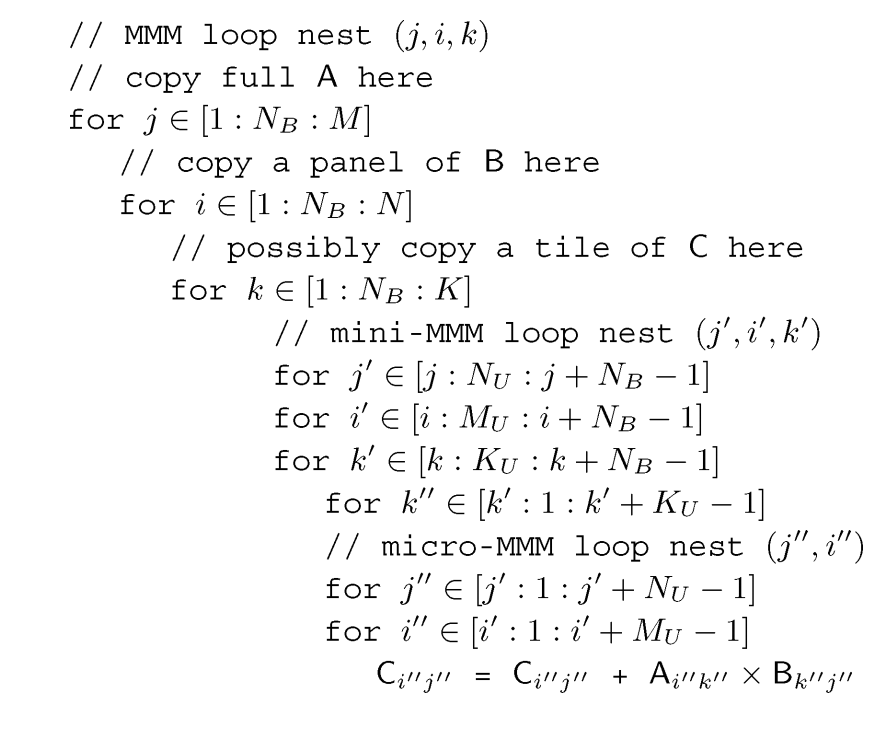
\includegraphics[width=0.4\textwidth]{images/ATLAS_code.png}
    \caption{}
  \end{subfigure}
  \begin{subfigure}[t]{1.0\linewidth}
    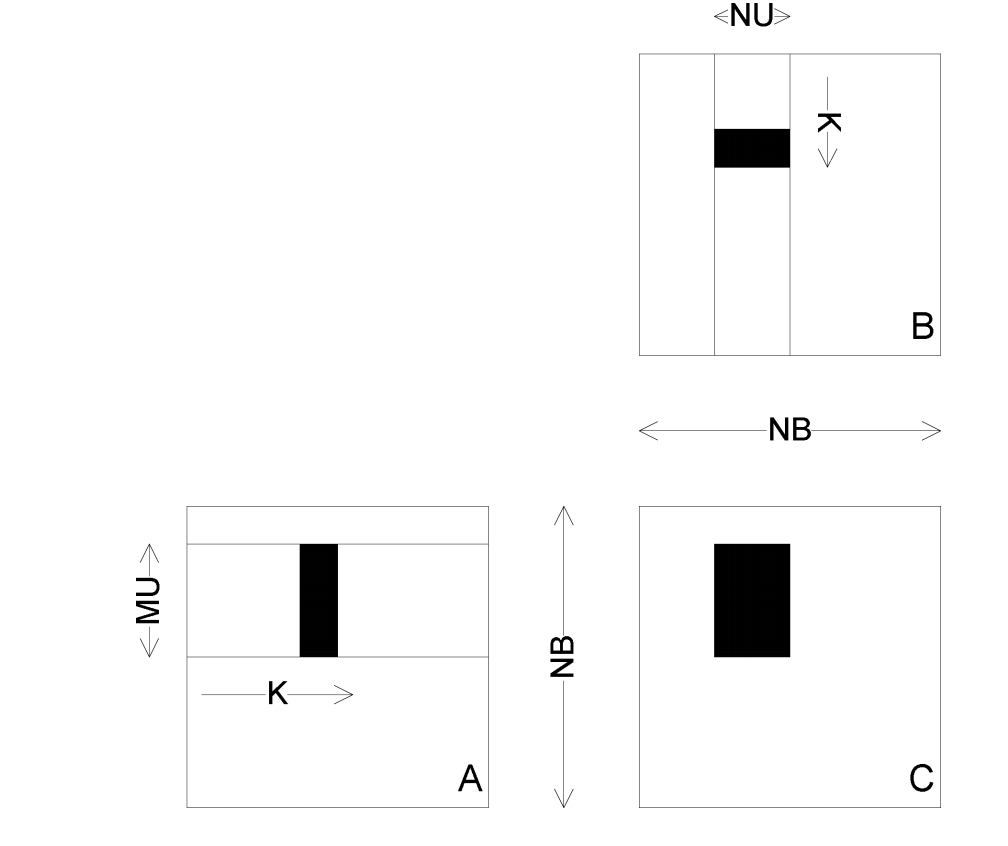
\includegraphics[width=0.4\textwidth]{images/ATLAS_pic.png}
    \caption{}
  \end{subfigure}
  \caption{Matrix multiplication tiled for L1 data cache and registers}
  \label{fig:design}
\end{figure*}



  \subsection{Capri approximation program}
  \label{sec:Capri_intro}
  a
